\chapter{Protocolo de autoconfiguración de direcciones propuesto}
%-----------------------------------
%   PROTOCOLO DE AUTOCONFIGURACIÓN DE DIRECCIONES PROPUESTO
%-----------------------------------
\label{ch:protocolo_autoconfiguracion_de_direcciones_propuesto}

Como se mencionó en el capítulo
\ref{ch:autoconfiguracion_de_direcciones_en_redes_descentralizadas}, para que
los vehículos puedan comunicarse a través de la red, necesitan tener una
dirección IP. Al no contar con un servidor DHCP en un VANET que se encargue de
asignar una dirección a cada vehículo, se requiere de un método que le permita
a cada vehículo obtener una dirección IP única de manera autónoma. Es por esto,
que se propone un protocolo de autoconfiguración de direcciones que permite que
cada vehículo y \textit{host} pueda obtener autónomamente una dirección IPv6., y
se describe en este capítulo

\section{Formación de las subredes}
%-----------------------------------
%   FORMACIÓN DE LAS SUBREDES
%-----------------------------------
\label{sec:formacion_de_subredes}

La razón por la que las direcciones IPv6 tienen una estructura jerárquica es
que, de este modo, los dispositivos que forman una red grande se pueden agrupar
para formar subredes, lo que facilita el enrutamiento. En las redes cableadas,
la jerarquización está determinada por la topología de la red, pero en una VANET
la topología cambia constantemente, por lo que se propone un método distinto
para agrupar a los vehículos en subredes.

Una dirección IPv6 se forma por dos partes (véase la sección
\ref{subsec:direccionamiento_ipv6}): el prefijo, que identifica a la subred, y
el identificador de la interfaz. Para que un vehículo pueda obtener una
dirección, primero debe saber a qué subred se va a unir. La formación de
subredes que se propone es dividir una región geográfica en regiones más
pequeñas, y agrupar a los vehículos que circulan en cada una de estas para
formar subredes. Para esto, se requiere que cada vehículo y \textit{host} pueda
conocer su ubicación geográfica.

Para definir los límites de las regiones, se utilizó un sistema de
geocodificación llamado Geohash, que permite representar regiones geográficas
mediante un código que se puede utilizar para generar el identificador de cada
subred para el prefijo de las direcciones IPv6. A continuación, se describe la
geocodificación Geohash.

\subsection{Geocodificación Geohash}
%-----------------------------------
%   GEOCODIFICACIÓN GEOHASH
%-----------------------------------
\label{subsec:geocodificacion_geohash}

En el sistema de geocodificación Geohash, se representa una ubicación o una
región geográfica con una cadena corta de letras y números. La longitud del
codigo determina la precisión de la ubicación. Además, esta codificación permite
saber si dos ubicaciones son cercanas analizando la longitud del prefijo común
entre sus códigos \cite{wiki:Geohash}.

Un código Geohash es una cadena binaria, que se convierte en una secuencia de
símbolos base 32. Estos símbolos se muestran en la tabla \ref{tab:base32}.

\begin{table}[th]
\centering
\caption{Codificación base 32.}
\label{tab:base32}
\begin{tabular}{c c}
\toprule
\tabhead{Binario} & \tabhead{Base 32} \\
\midrule
00000 & 0 \\
00001 & 1 \\
00010 & 2 \\
00011 & 3 \\
00100 & 4 \\
00101 & 5 \\
00110 & 6 \\
00111 & 7 \\
01000 & 8 \\
01001 & 9 \\
01010 & b \\
01011 & c \\
01100 & d \\
01101 & e \\
01110 & f \\
01111 & g \\
\bottomrule
\end{tabular}
\quad
\begin{tabular}{c c}
\toprule
\tabhead{Binario} & \tabhead{Base 32} \\
\midrule
10000 & h \\
10001 & j \\
10010 & k \\
10011 & m \\
10100 & n \\
10101 & p \\
10110 & q \\
10111 & r \\
11000 & s \\
11001 & t \\
11010 & u \\
11011 & v \\
11100 & w \\
11101 & x \\
11110 & y \\
11111 & z \\
\bottomrule
\end{tabular}
\end{table}

Para formar un código Geohash, se divide toda la superficie de la Tierra en 32
celdas (figura \ref{fig:geohash1}), y cada una tiene asignado un símbolo. Se
elige la región que contiene la ubicación/región de interés y se agrega el
símbolo correspondiente al código. La región seleccionada se divide en 32
celdas (figura \ref{fig:geohash2}), y se selecciona la celda que contiene la
ubicación/región de interés, y su símbolo se agrega al código. Este proceso se
repite hasta obtener la precisión necesaria. Nótese que, mientras más largo sea
el prefijo común entre dos códigos, más cercanas entre sí son las ubicaciones
que representan. En el apédice \ref{app:b} se muestra un algoritmo para generar
un código Geohash a partir de una ubicación geográfica.

\begin{figure}[th!]
\centering
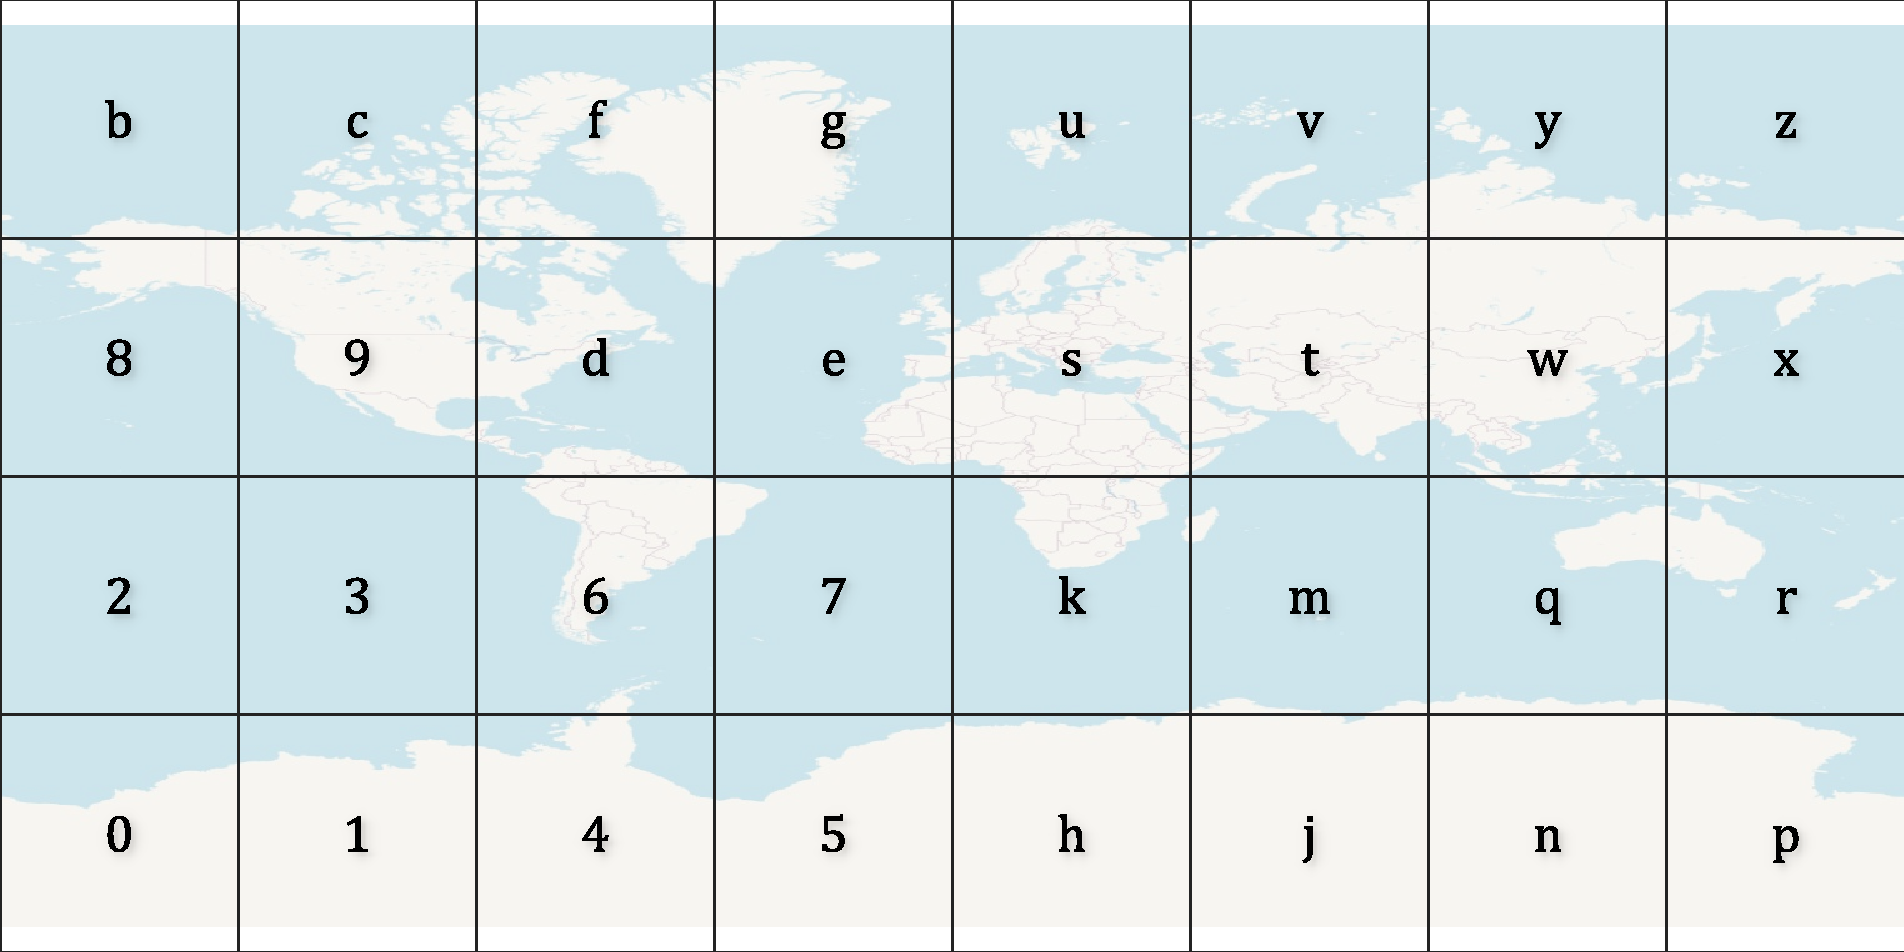
\includegraphics[width=0.85\textwidth]{geohash1} 
\decoRule
\caption[Códio Geohash de longitud 1]{Códio Geohash de longitud 1.}
\label{fig:geohash1}
\end{figure}

\begin{figure}[th!]
\centering
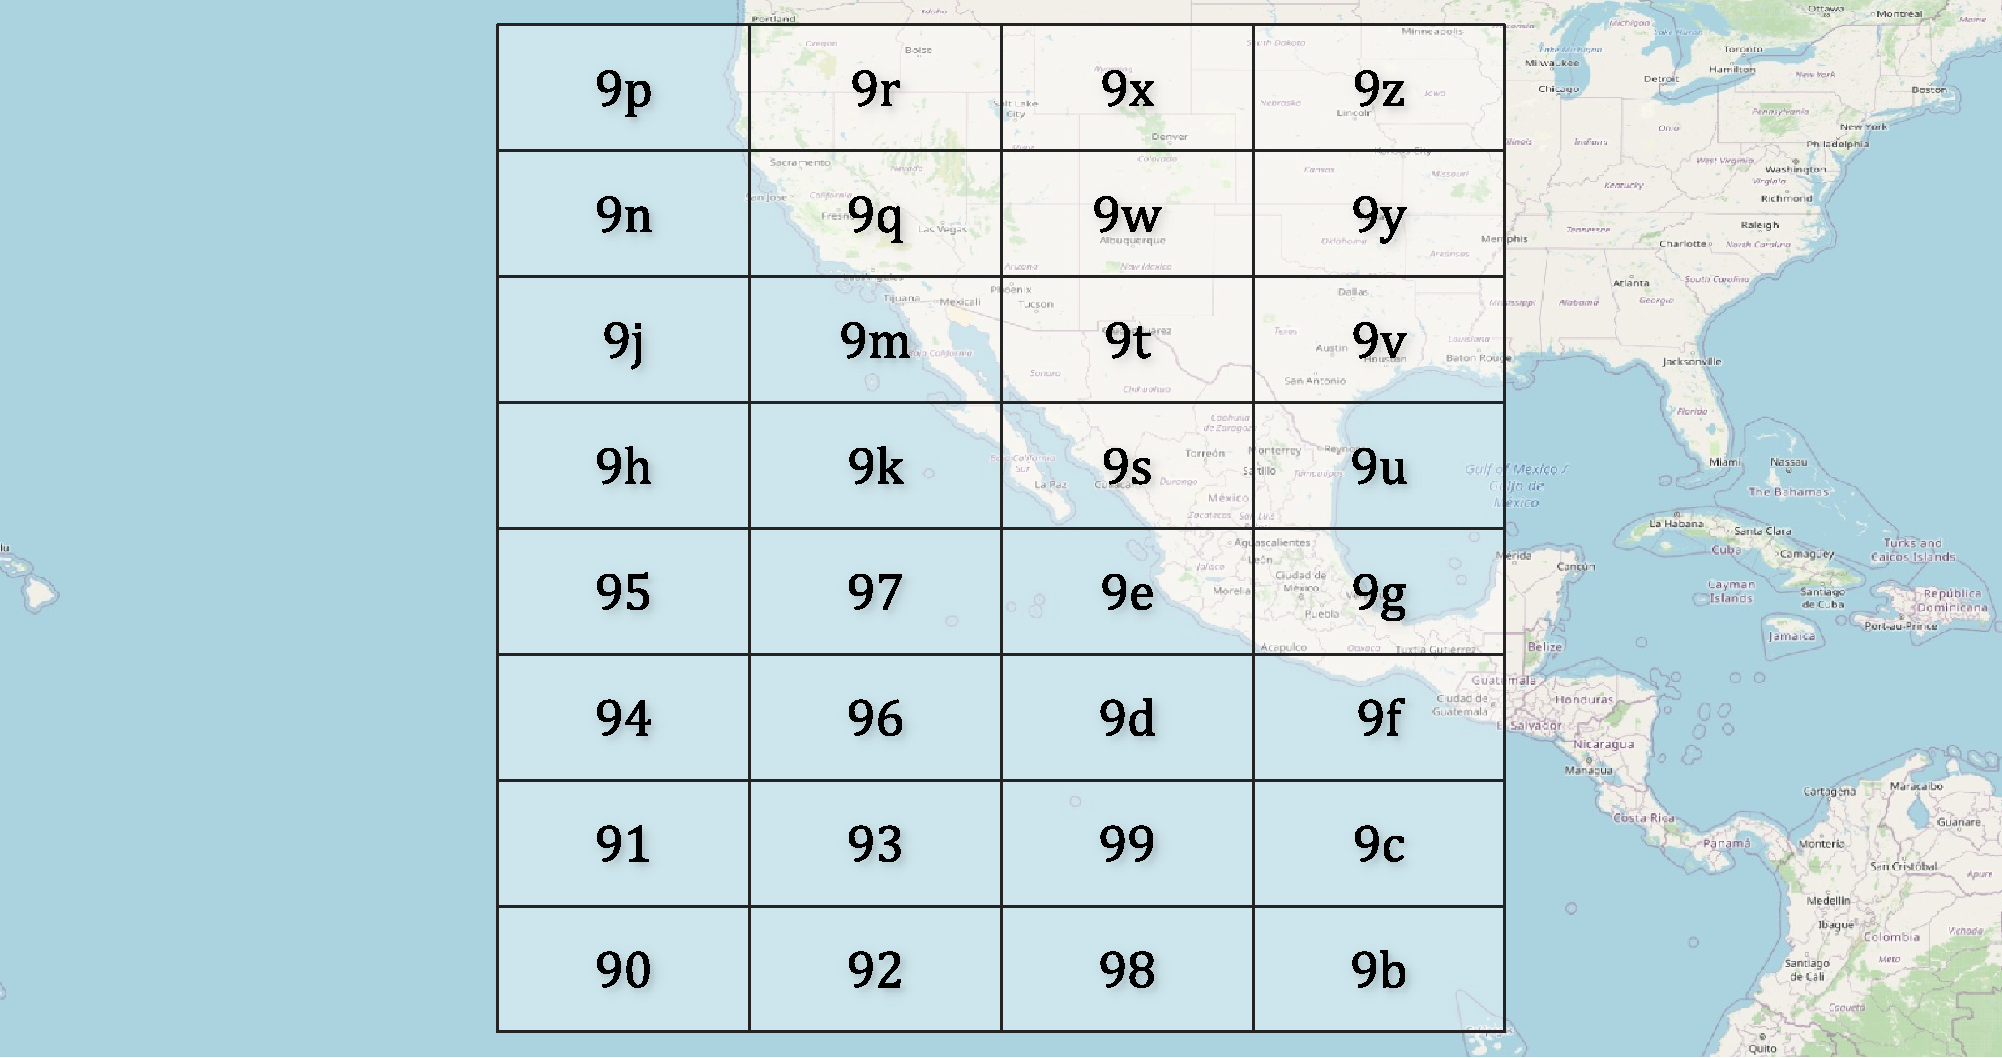
\includegraphics[width=0.85\textwidth]{geohash2}
\decoRule
\caption[Códio Geohash de longitud 2]{Códio Geohash de longitud 2.}
\label{fig:geohash2}
\end{figure}

Un mismo código se puede interpretar con una región o como una ubicación
puntual, en cuyo caso, se considera el centro de la región. En la tabla
\ref{tab:tamaño_celdas_geohash} se muestra el tamaño aproximado de las celdas
que se obtienen de acuerdo a la longitud del código. Se debe considerar que el
tamaño de las celdas es más pequeño a medida que la latitud se aleja del
ecuador.

\begin{table}[th]
\caption{Tamaño de las celdas para diferentes longitudes de código
\cite{GeohashBolivia}.}
\label{tab:tamaño_celdas_geohash}
\centering
\begin{tabular}{c c r r}
\toprule
\tabhead{Longitud del código} & & \tabhead{Ancho} & \tabhead{Alto}\\
\midrule
1 & $\leq$ & 5,000 km & 5,000 km\\
2 & $\leq$ & 1,250 km & 625 km\\
3 & $\leq$ & 156 km & 156 km\\
4 & $\leq$ & 39.1 km & 19.5 km\\
5 & $\leq$ & 4.89 km & 4.89 km\\
6 & $\leq$ & 1.22 km & 0.61 km\\
7 & $\leq$ & 153 m & 153 m\\
8 & $\leq$ & 38.2 m & 19.1 m\\
9 & $\leq$ & 4.77 m & 4.77 m\\
10 & $\leq$ & 1.19 m & 0.596 m\\
11 & $\leq$ & 149 mm & 149 mm\\
12 & $\leq$ & 37.2 mm & 18.6 mm\\
\bottomrule\\
\end{tabular}
\end{table}

A partir de aquí, se llamará código \textbf{Geohash-\textit{n}} a un código
Geohash de longitud \textit{n}. También, se entenderá como \textbf{región
Geohash} o \textbf{ubicación Geohash} a una región o ubicación representada por
un código Geohash.

\subsection{Subredes Geohash}
%-----------------------------------
%   SUBREDES GEOHASH
%-----------------------------------
\label{subsec:subredes_geohash}

Utilizando códigos Geohash, se definen las regiones con las que se formarán las
subredes, que se denominan \textbf{subredes geohash}. Estas subredes se forman
por los vehículos que se encuentran dentro de los límites de la región. Pero
falta determinar cuál es el mejor tamaño para estas regiones.

Si las regiones fueran muy grandes, habría muy pocas subredes con muchos
vehículos cada una, por lo que la jerarquización de direcciones sería muy débil,
y no ayudaría a simplificar el enrutamiento. Por ejemplo, en la figura
\ref{fig:region_geohash5} se puede notar que las regiones Geohash-5 abarcan un
área muy grande, aproximadamente de 4.89x4.89km, seún la tabla
\ref{tab:tamaño_celdas_geohash}, que es un ejemplo de este caso. Por otra parte,
si las regiones fueran muy pequeñas, habría muchas subredes con muy pocos
vehículos. En la figura \ref{fig:region_geohash7} se observa que las regiones
Geohash-7 son tan pequeñas, que algunas apenas abarcan un segmento de alguna
calle, en cuyo caso, podría llegar a haber regiones sin ningún vehículo. Además,
algunos pares de celdas adyacentes no cuentan con algún segmento de calle que
las conecte, por lo que los vehículos no podrían pasar de una región a otra.

Por otro lado, las regiones Geohash-6 tienen un tamaño más razonable, como se
puede ver en la figura \ref{fig:region_geohash6}. Según la tabla
\ref{tab:tamaño_celdas_geohash}, las dimensiones de estas regiones son de
1.22x0.61km, aproximadamente, y todas tienen al menos un segmento de calle que
las conecta con sus regiones asyacentes. Es por esto, que eligió que las
regiones para las subredes serán definidas por códigos Geohash-6.

\begin{figure}[th!]
\centering

\begin{subfigure}{\textwidth}
\centering
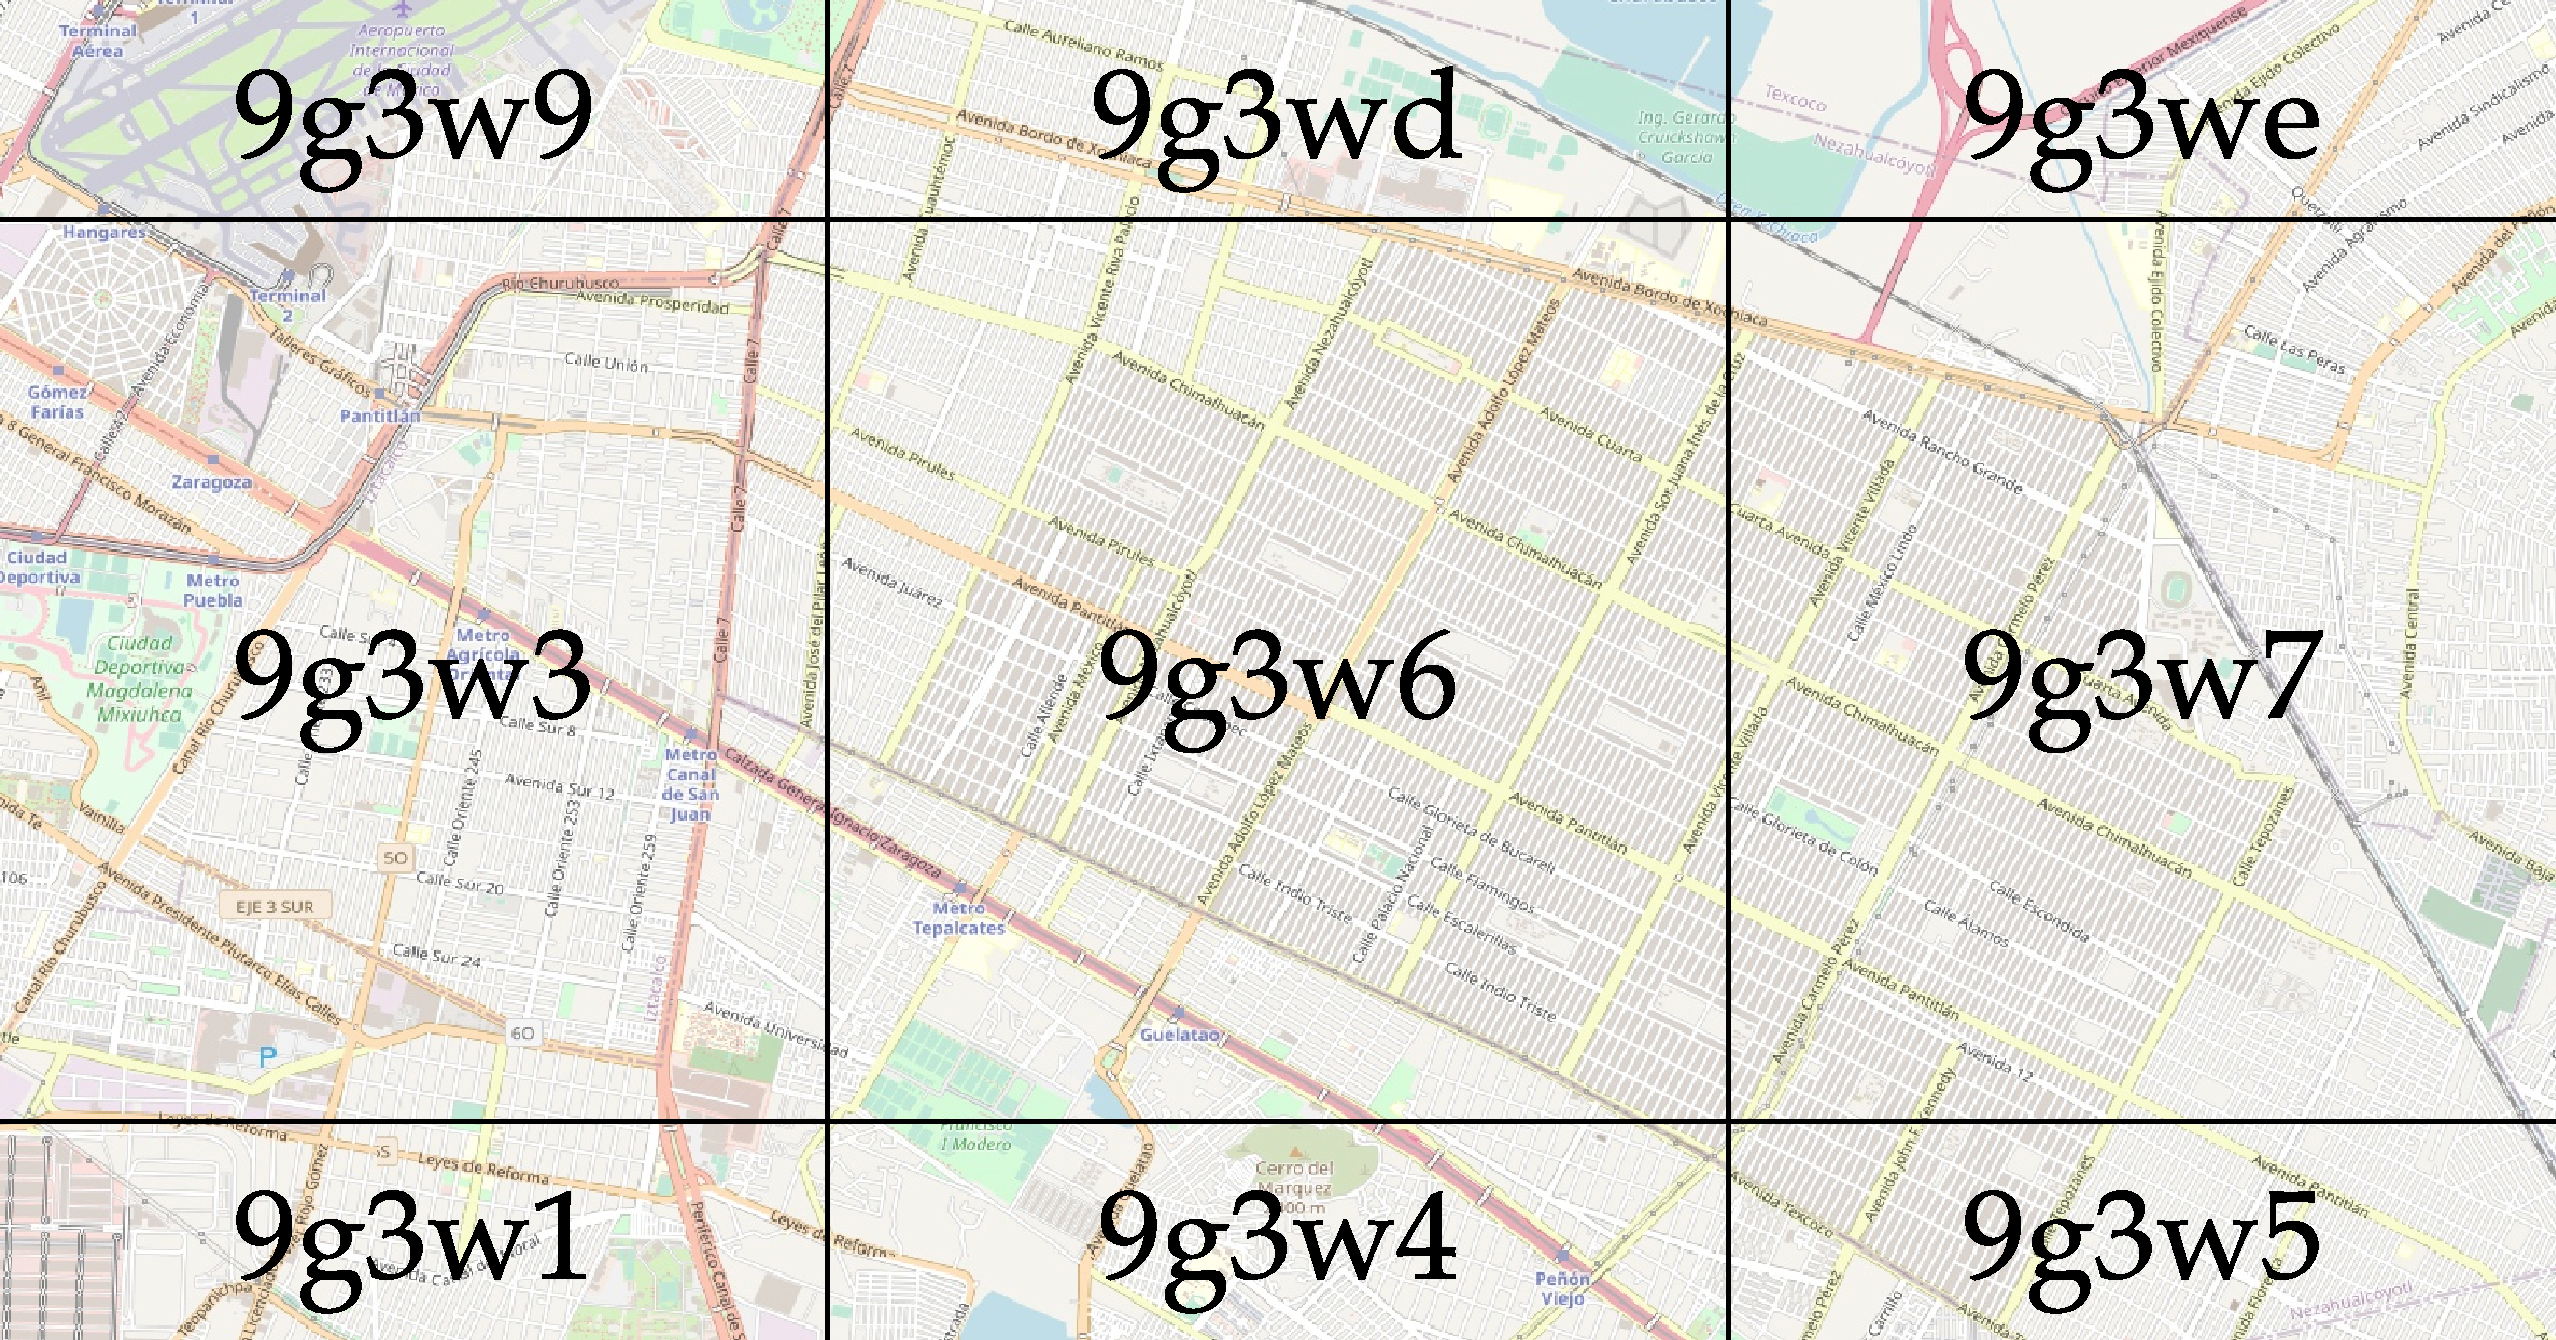
\includegraphics[height=4cm]{region_geohash5} 
\caption[Regiones Geohash-5]{Regiones Geohash-5.}
\label{fig:region_geohash5}
\end{subfigure}

\vspace{0.5cm}

\begin{subfigure}{\textwidth}
\centering
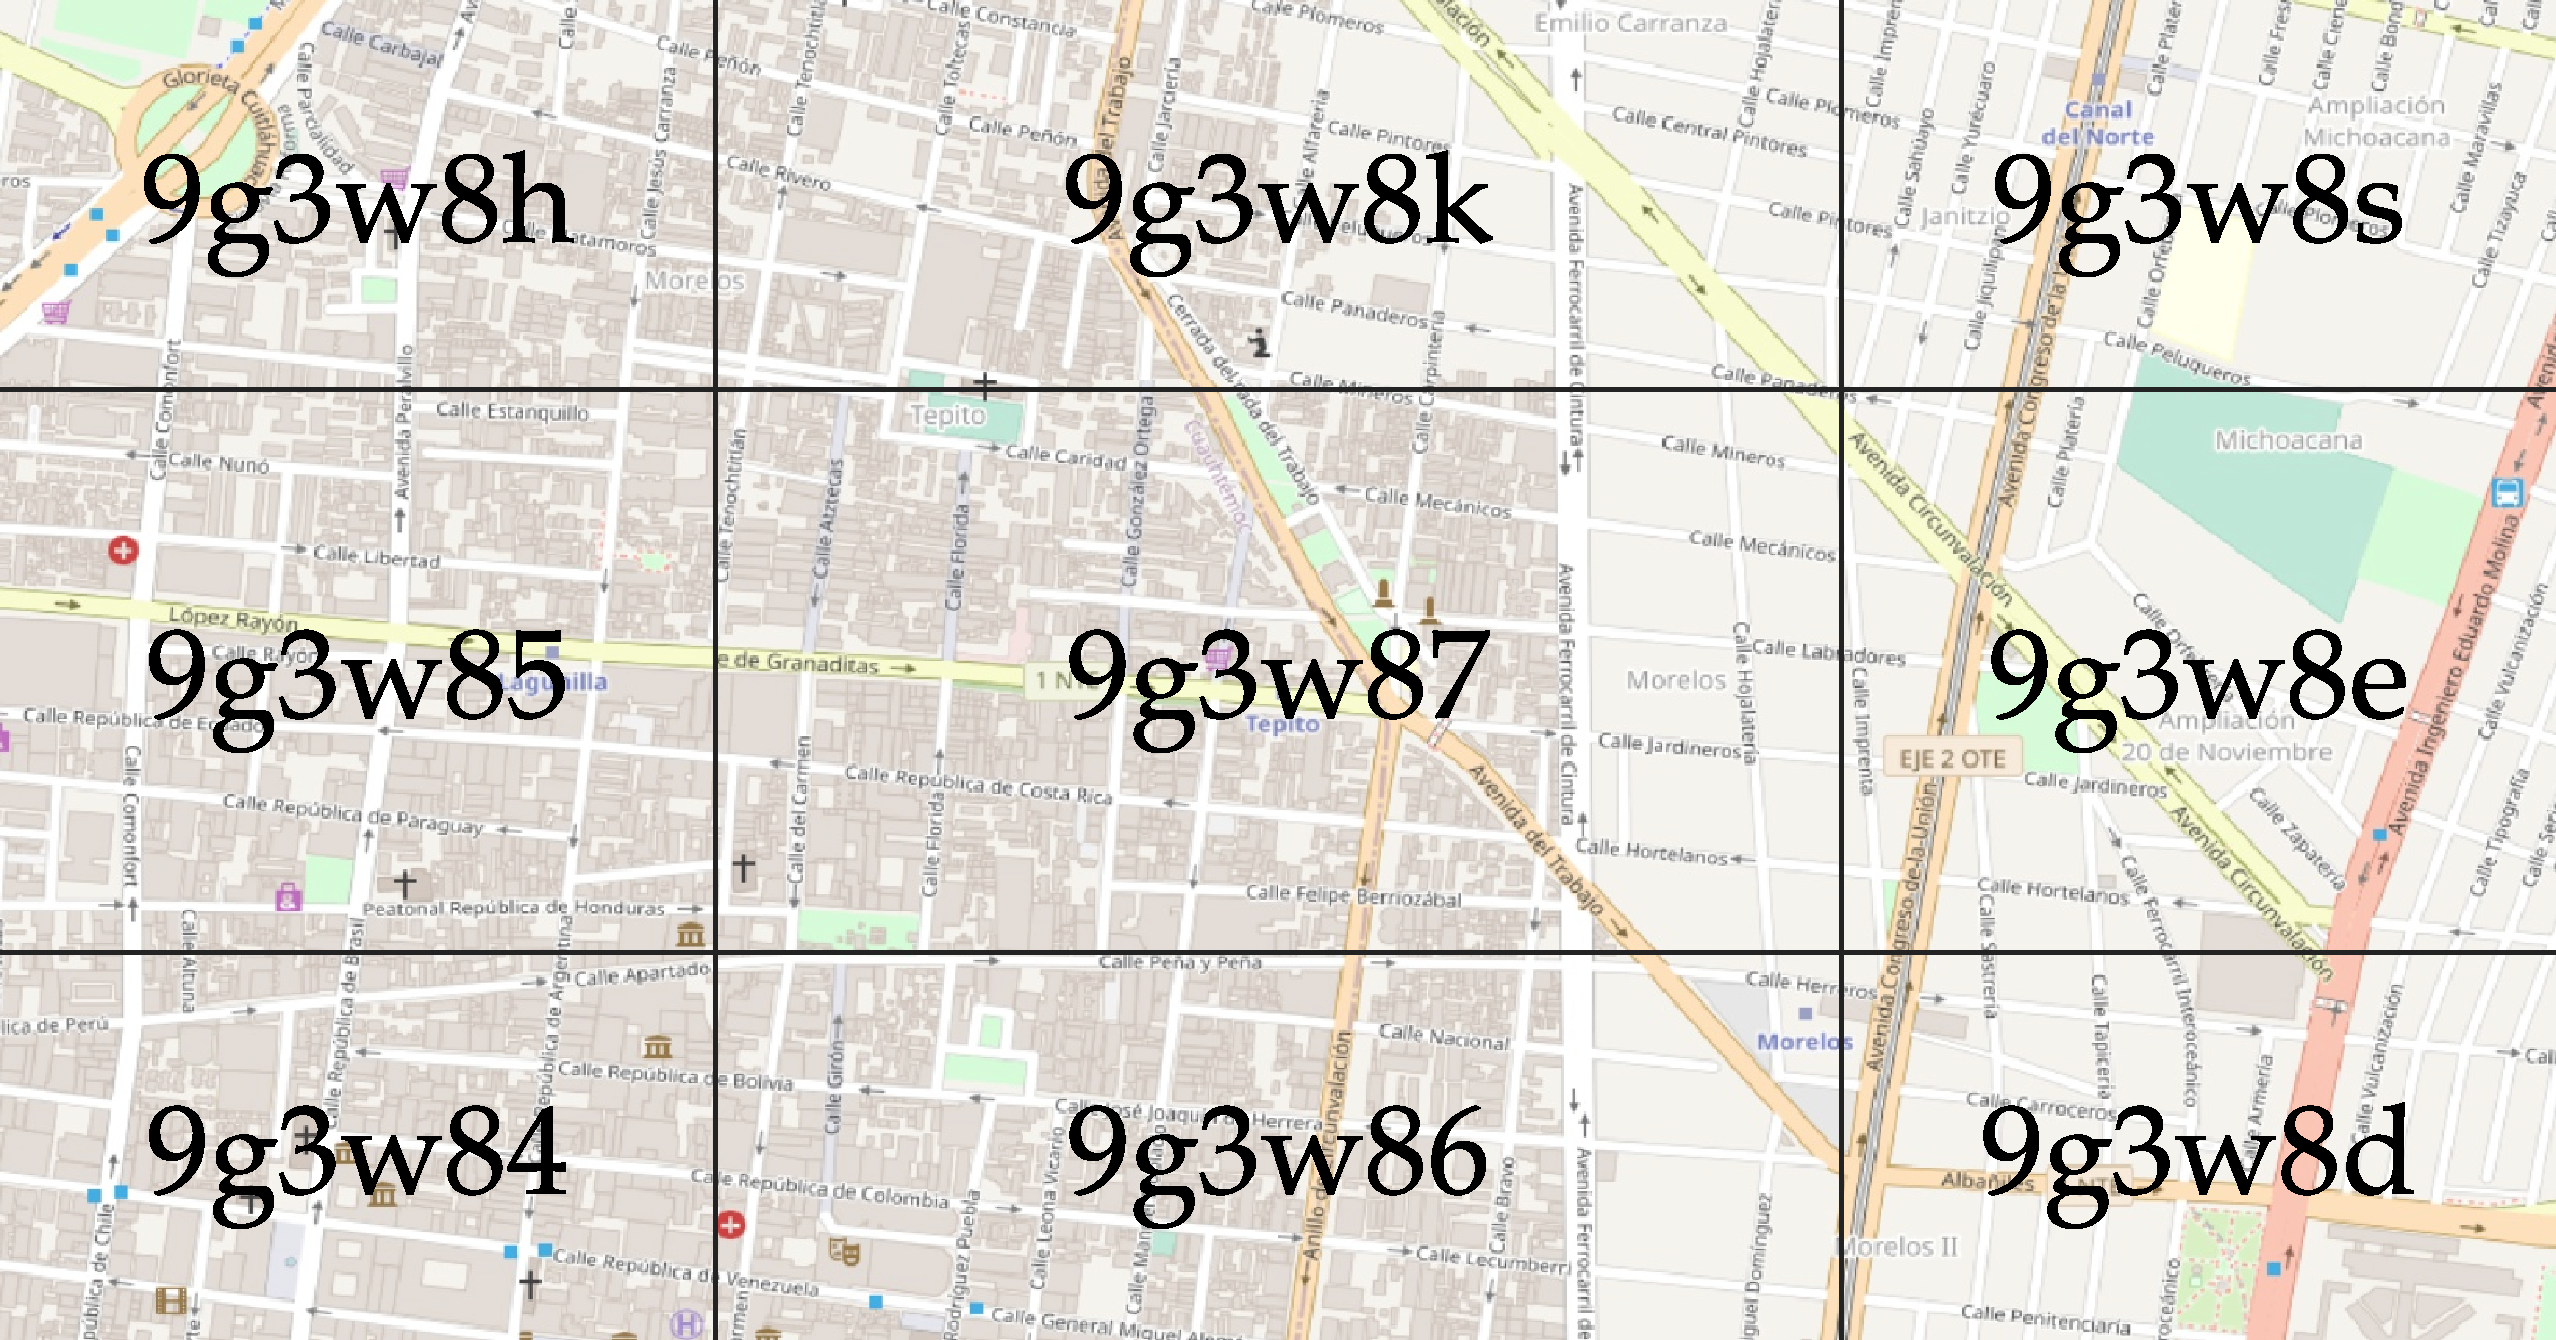
\includegraphics[height=4cm]{region_geohash6} 
\caption[Regiones Geohash-6]{Regiones Geohash-6.}
\label{fig:region_geohash6}
\end{subfigure}

\vspace{0.5cm}

\begin{subfigure}{\textwidth}
\centering
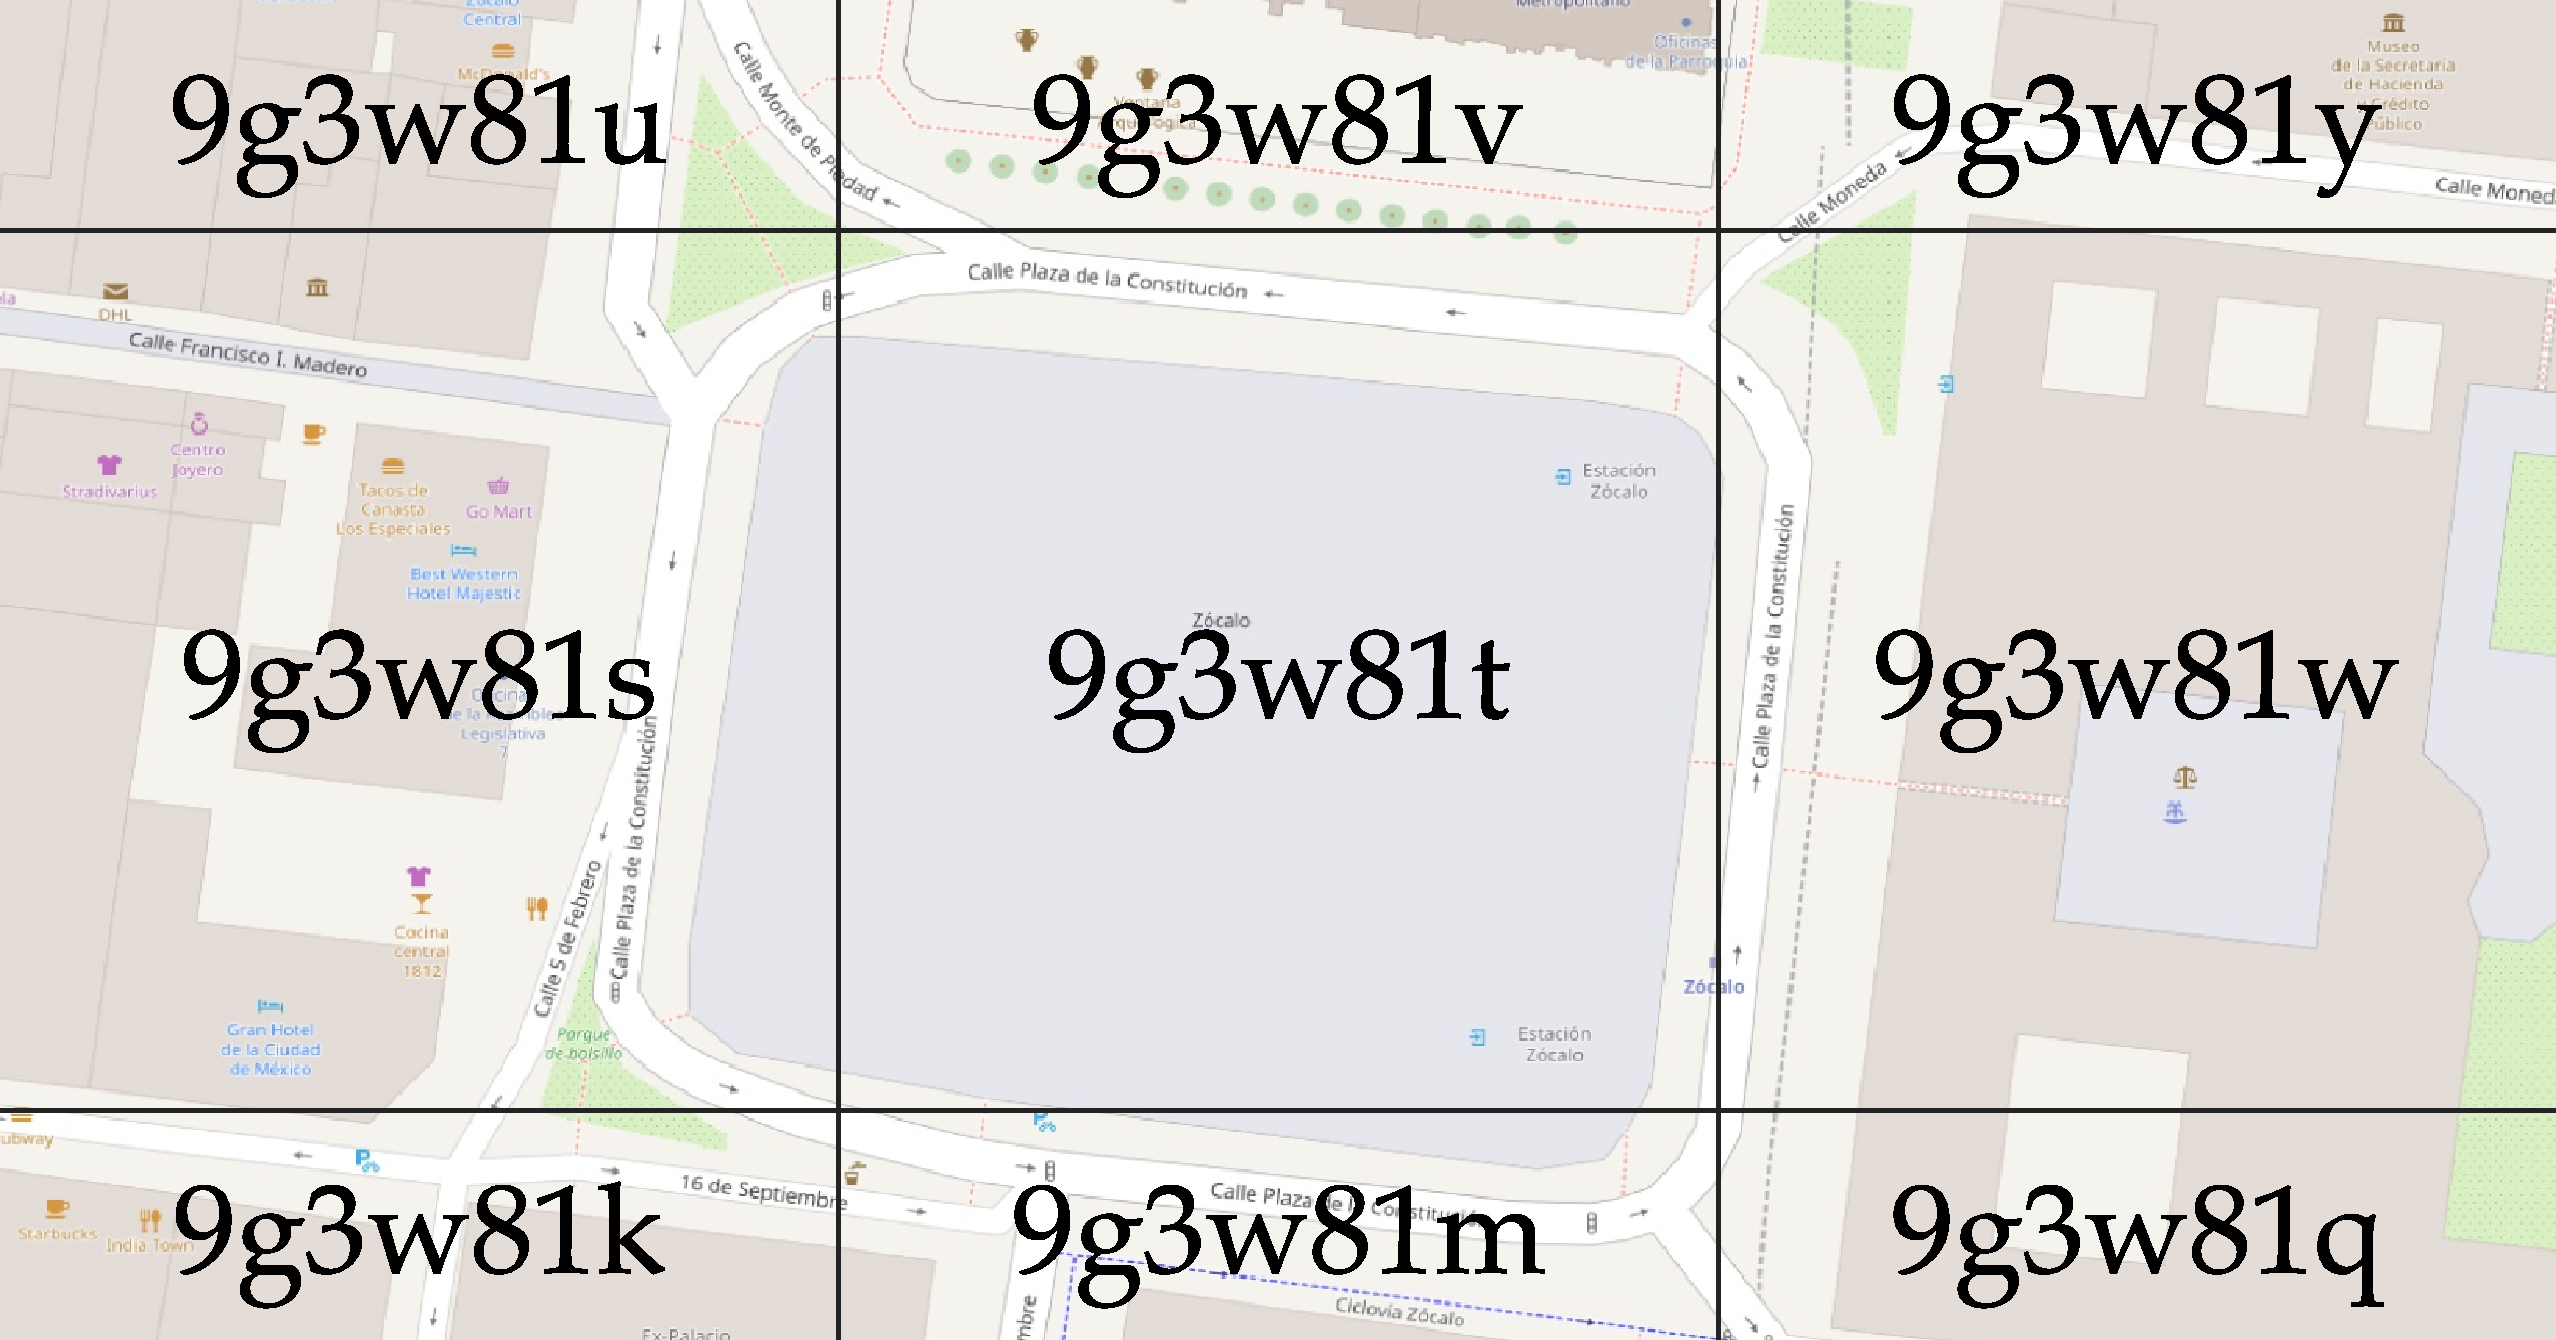
\includegraphics[height=4cm]{region_geohash7} 
\caption[Regiones Geohash-7]{Regiones Geohash-7.}
\label{fig:region_geohash7}
\end{subfigure}

\vspace{0.5cm}

\decoRule
\caption[Tamaños de regiones Geohash]{Tamaños de regiones Geohash.}
\label{fig:tamaños_geohash}

\end{figure}

\section{Formato de las direcciones IPv6}
%-----------------------------------
%   FORMATO DE LAS DIRECCIONES IPV6
%-----------------------------------
\label{sec:formato_direcciones_ipv6}

Cuando un vehículo o \textit{host} necesita transmitir un paquete hacia otro,
debe conocer su dirección \textit{unicast} para referiste a exclusivamente a
este, por lo que cada uno debe tener forzosamente una dirección
\textit{unicast}. Por otro lado, los protocolos de enrutamiento requieren que
todos los nodos de una red compartan mensajes con todos sus vecinos, y el
protocolo propuesto no es la excepción. Es por esto que todos los vehículos y
\textit{hosts} tengan también una dirección \textit{multicast}.

Tanto las direcciones \textit{unicast} como \textit{multicast} deben contener el
identificador de la subred. Cuando un nodo conoce su ubicación, con ella puede
calcular el código Geohash correspondiente. Todos los nodos que se encuentren en
la misma región obtendrán un código Geohash con los mismos primeros 6 símbolos,
que forman el código Geohash-6 que identifica la subred en la que se
encuentran. De este modo, todos pueden obtener directamente el identificador de
la subred en la que se encuentran.

El protocolo de autoconfiguración de direcciones define reglas para que cada
nodo de la red pueda generar sus propias direcciones y configurarse sin ayuda de
los demás. A continuación, se describe cómo se forman estas direcciones.

\subsection{Direcciones IPv6 \textit{unicast}}
%-----------------------------------
%   DIRECCIONES UNICAST
%-----------------------------------
\label{subsec:direcciones_unicast}

El protocolo IPv6 define diferentes tipos de direcciones \textit{unicast}, que
se describen a continuación \cite{CiscoIpv62011}:

\keyword{Dirección global agregable} -- Estas direcciones tienen un prefijo de
enrutamiento global de 48 bits que comienza con \code{2000::/3}. En seguida,
tiene un identifiador de subred de  16 bits, y al final el identificador del
nodo de 64 bits. Su asignación depende de la Autoridad de Asignación de Números
de Internet (IANA) y los proveedores de servicio de Internet (ISPs).

\keyword{Dirección local de enlace} --  Se pueden configurar automáticamente con
el prefijo \code{FE80::/10} y el identificador de la interfaz con el formato
EUI-64 (\ref{app:a}). Se usa para el protocolo de descubrimiento de vecinos y
el proceso de autoconfiguración sin estado. Los paquetes destinados a este tipo de
dirección no son enrutados.

\keyword{Dirección compatible con IPv4} -- Son direcciones que comienzan con el
prefijo \code{::/96} seguido de una dirección IPv4 de 32 bits. Se asignan a
nodos que sportan tanto IPv4 como IPv6.

\keyword{Dirección local única} -- Inician con el prefijo \code{FC00::/7}. Son
direcciones únicas globalmente, y son destinadas únicamente para comunicación
local; es decir, no se enrutan hacia Internet. Su asignación no depende del ISP
o de alguna otra entidad reguladora.

Debido a que no hay restricciones para la utilización de direcciones locales
únicas, este es el tipo de dirección \textit{unicast} que se usarán para
identificar a los nodos. La figura \ref{fig:formato_direccion_unicast}
muestra el formato de una dirección local única \cite{CiscoIpv62011}.

\begin{figure}[th!]
\centering
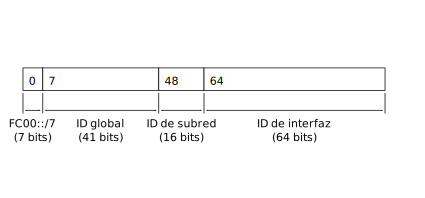
\includegraphics{formato_direccion_unicast}
\decoRule
\caption[Formato de una dirección local única]{Formato de una dirección
local única.}
\label{fig:formato_direccion_unicast}
\end{figure}

El formato de las direcciones \textit{unicast} se muestra en la figura
\ref{fig:formato_direccion_unicast_geohash}, y se conforma de la siguiente
manera:

\begin{figure}[th!]
\centering
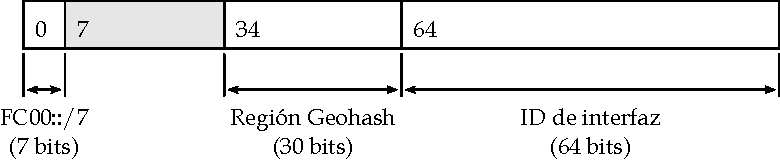
\includegraphics{formato_direccion_unicast_geohash}
\decoRule
\caption[Formato de una dirección \textit{unicast} Geohash]{Formato de una
dirección \textit{unicast} Geohash.}
\label{fig:formato_direccion_unicast_geohash}
\end{figure}

\keyword{Bits 0 - 6} -- Prefijo \code{FC00::/7}, que indica que se trata de
una dirección local única.

\keyword{Bits 7 - 33} -- No se usan; valen 0.

\keyword{Bits 34 - 63} -- Código Geohash de la subred.

\keyword{Bits 64 - 127} -- Identificador de la interfaz en el formato
EUI-64.

\section{Direcciones IPv6 \textit{multicast}}
%-----------------------------------
%   DIRECCIONES IPV6 MULTICAST
%-----------------------------------
\label{subsec:direcciones_ipv6_multicast}

En el protocolo IPv6, una dirección \textit{multicast} se forma por dos partes:
el prefijo \code{FF02::/16} y el identificador del grupo \textit{multicast},
como se muestra en la figura \ref{fig:formato_direccion_multicast}.

\begin{figure}[th!]
\centering
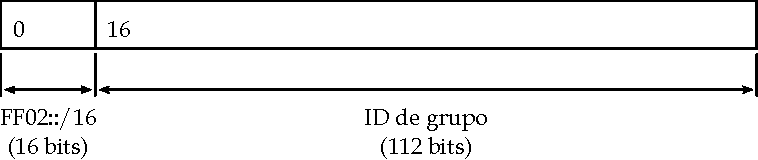
\includegraphics{formato_direccion_multicast}
\decoRule
\caption[Formato de una dirección \textit{multicast}]{Formato de una dirección
\textit{multicast}.}
\label{fig:formato_direccion_multicast}
\end{figure}

El formato de las direcciones \textit{multicast} se muestra en la figura
\ref{fig:formato_direccion_multicast_geohash}, y se conforma de la siguiente
manera:

\begin{figure}[th!]
\centering
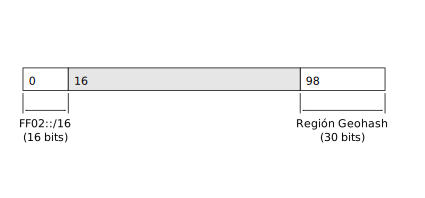
\includegraphics{formato_direccion_multicast_geohash}
\decoRule
\caption[Formato de la dirección \textit{multicast} para cada región]{Formato de
la dirección \textit{multicast} para cada región.}
\label{fig:formato_direccion_multicast_geohash}
\end{figure}

\keyword{Bits 0 - 15} -- Prefijo \code{FF02::/16}, que indica que se trata
de una dirección multicast.

\keyword{Bits 16 - 97} -- No se usan; se fijan en 0.

\keyword{Bits 98 - 127} -- Código Geohash de la subred.

\section{Cambio de subred}
%-----------------------------------
%   CAMBIO DE SUBRED
%-----------------------------------
\label{sec:cambio_subred}

Para que un vehículo o \textit{host} se pueda configurar para unirse a una
subred, lo único que necesita es conocer su ubicación geográfica, y con ella
puede generar sus direcciones \textit{unicast} y \textit{multicast}, como se
describió anteriormente. Sin embargo, los vehículos deben seguir ciertas reglas
cuando se mueven de una subred a otra.

Cuando un vehículo entra a una nueva subred, no es conveniente que deseche las
direcciones correspondientes a la subred anterior, ya que, como se explicará en
el siguiente capítulo, el protocolo de enrutamiento requiere que se comunique
con vehículos de ambas subredes. Es por esto que necesita mantener sus
direcciones \textit{unicast} y \textit{multicast} de la subred anterior por un
tiempo después de que entra a otra subred mientras se encuentra en una región
llamada \textbf{región \textit{gateway}}, que se muestra de color gris en la
figura \ref{fig:region_gateway}. Un vehículo que se encuentra en una región
\textit{gateway}, se denomina simplemente \textbf{gateway}, ya que funciona como
un enlace entre dos subredes adyacentes.

\begin{figure}[th]
\centering
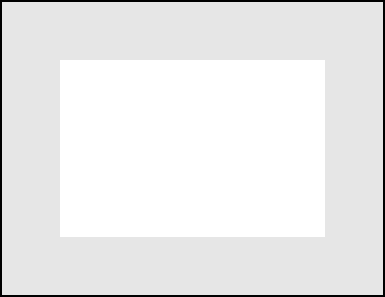
\includegraphics{region_gateway}
\decoRule
\caption[Región \textit{gateway}]{Región \textit{gateway}.}
\label{fig:region_gateway}
\end{figure}

En la figura \ref{fig:cambio_subred}, se muestran dos subredes adyacentes y las
fronteras de sus regiones, además de la ubicación de un vehículo en cuatro
instantes de tiempo. En el tiempo $t_0$, se encuentra en la región 1, pero fuera
de la región \textit{gateway}, por lo que únicamente forma parte de esta. En el
tiempo $t_1$, está en la región \textit{gateway} de la región 1, así que
también debe formar parte de la subred 2. En el tiempo $t_2$, entró a la región
2, y se encuentra en la región \textit{gateway} de esta. En este caso, también
debe formar parte de ambas subredes. En el tiempo $t_3$, se encuentra en la
región 2, pero fuera de la región \textit{gateway}, así que únicamente forma
parte de la subred 2.

\begin{figure}[th]
\centering
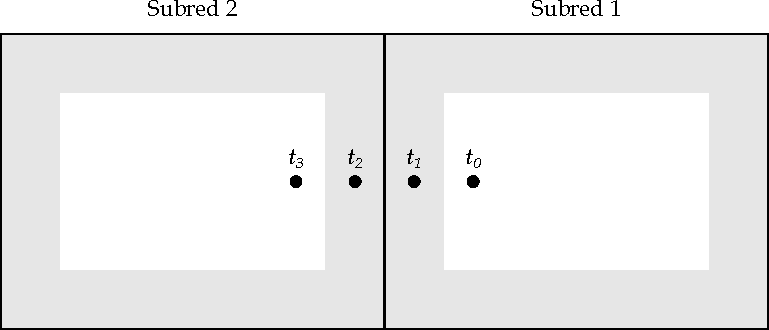
\includegraphics{cambio_subred}
\decoRule
\caption[Cambio de subred de un vehículo]{Cambio de subred de un vehículo.}
\label{fig:cambio_subred}
\end{figure}
